\section{Chemical bonding}
\subsection{Electronegativity and bonding}
\begin{point}
Define electronegativity as the power of an atom to attract electrons to itself
\end{point}
Self explanatory.

\begin{point}
Explain the factors infuencing the electronegativities of the elements in terms
of nuclear charge, atomic radius and shielding by inner shells and sub-shells
\end{point}
Electronegativity is influenced by the following:
\begin{itemize}
	\item Nuclear charge: Atoms with a greater positive nuclear charge have a 
		greater electronegativity, as they can pull attract electrons to 
		themselves.
	\item Atomic radius: The larger the atomic radius, the smaller the 
		electronegativity, since it is harder to cause attraction over a larger
		distance.
	\item Shielding: The greater the number of inner electron shells and sub
		shells, the lower the effective nuclear charge on bonding electrons as
		these inner electrons are repelling the outer ones.
\end{itemize}

\begin{point}
State and explain the trends in electronegativity across a period and down a
group of the Periodic Table
\end{point}
Electronegativity increases across a period from Group 1 to Group 17, and it
decreases down each group.

Across a period, nuclear charge increases whilst shielding remains the same,
as does atomic radius, increasing electronegativity.

Down a group, atomic radius and shielding increase, as down nucleaer charge,
however, the increase in shielding is the most influential of these factors and 
this is what causes the decrease in electronegativity.

\begin{point}
Use the differences in Pauling electronegativity values to predict the 
formation of ionic and covalent bonds (the presence of covalent character in 
some ionic compounds will not be assessed) (Pauling
electronegativity values will be given where necessary)
\end{point}
Every atom has its own electronegativity, which is measured in the Pauling
electronegativity scale. Note that carbon and hydrogen have low 
electronegativities. The value of electronegativity is denoted $N_\text{p}$

For elements chemically bonded, the differences in their electronegativities
can be used to predict the ionic or covalent character of their bonds. A
high difference ($>2.0$) signifies an ionic bond, whereas a lower difference
($<1.0$) signifies a covalent bond. A zero value shows absence of any ionic
character and any value between 1 and 2 shows that the compound is not entirely
covalent and has some ionic character.

\subsection{Ionic bonding}
\begin{point}
Define ionic bonding as the electrostatic attraction between oppositely charged
ions (positively charged cations and negatively charged anions)}
\end{point}
Self explanatory.

\begin{point}
Describe ionic bonding including the examples of sodium chloride, magnesium
oxide and calcium fluoride
\end{point}
Ionic bonds form between metals and non-metals, where the metallic element 
loses its valence electrons, which are gained by the non-metal, producing a
metal cation and a non-metal anion which bond together via electrostatic
attraction.

Consider sodium chloride, \ce{NaCl}, which consists of the ions \ce{Na+} and
\ce{Cl-}, formed when the Na atom loses its valence electron which is gained
by the Cl atom. We can represent this in a dot and cross diagram:

$$
\vcenter{
\hbox{
\begin{tikzpicture}[baseline=(base)]
	\node (base) at (0,0) {};
	\draw (0, 0) circle (0.5);
	\node at (0, 0) {Na};
	\node at (0, 0.5) {$\times$};
	\node at (0.9, 0) {\rightarrow};
	
	% Bracketed ion
	\node at (2.25, 0) {
		$\left[
		\vcenter{
		\hbox{
		\begin{tikzpicture}
			\draw (0, 0) circle (0.5);
			\node at (0, 0) {Na};
		\end{tikzpicture}
		}}
		\right]^{+}$
	};

	\node at (3.5, 0) {$+$};
	\node at (4, 0) {$\times^-$};
\end{tikzpicture}
}}
$$

$$
\vcenter{
\hbox{
\begin{tikzpicture}[baseline=(base)]
	\node (base) at (0,0) {};

	% Chlorine atom
	\draw (0.1, 0) circle (0.5);
	\node at (0.1, 0) {Cl};

	% Incoming electron
	\node at (-0.9, 0) {$\times^- +$};
	\node at (0.9, 0) {\rightarrow};

	\node at (0.6, -0.1) {$\bullet$};
	\node at (0.6, 0.1) {$\bullet$};
	\node at (-0.4, 0.1) {$\bullet$};
	\node at (-0.4, -0.1) {$\bullet$};
	\node at (0, -0.5) {$\bullet$};
	\node at (0.2, -0.5) {$\bullet$};
	\node at (0, 0.5) {$\bullet$};

	% Bracketed ion
	\node at (2.25, 0) {
		$\left[
		\vcenter{
		\hbox{
		\begin{tikzpicture}
			\draw (0, 0) circle (0.5);
			\node at (0, 0) {Cl};
			\node at (0.5, -0.1) {$\bullet$};
			\node at (0.5, 0.1) {$\bullet$};
			\node at (-0.5, 0.1) {$\bullet$};
			\node at (-0.5, -0.1) {$\bullet$};
			\node at (0.1, -0.5) {$\bullet$};
			\node at (-0.1, -0.5) {$\bullet$};
			\node at (0.1, 0.5) {$\bullet$};
			\node at (-0.1, 0.5) {$\times$};
		\end{tikzpicture}
		}}
		\right]^-$
	};
\end{tikzpicture}
}}
$$

Thus a molecule of \ce{NaCl} is shown as follows in a dot and cross diagram
$$
\left[
	\vcenter{
		\hbox{
			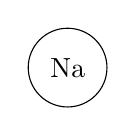
\begin{tikzpicture}
				\draw (0, 0) circle (0.5);
				\node at (0, 0) {Na};
			\end{tikzpicture}
	}}
\right]^{+}
\left[
\vcenter{
	\hbox{
		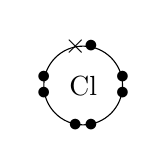
\begin{tikzpicture}
			\draw (0, 0) circle (0.5);
			\node at (0, 0) {Cl};
			\node at (0.5, -0.1) {$\bullet$};
			\node at (0.5, 0.1) {$\bullet$};
			\node at (-0.5, 0.1) {$\bullet$};
			\node at (-0.5, -0.1) {$\bullet$};
			\node at (0.1, -0.5) {$\bullet$};
			\node at (-0.1, -0.5) {$\bullet$};
			\node at (0.1, 0.5) {$\bullet$};
			\node at (-0.1, 0.5) {$\times$};
		\end{tikzpicture}
}}\right]^-
$$

Given below are the cases for \ce{MgO} and \ce{CaF2}

$$
\left[
	\vcenter{
		\hbox{
			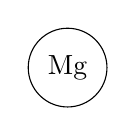
\begin{tikzpicture}
				\draw (0, 0) circle (0.5);
				\node at (0, 0) {Mg};
			\end{tikzpicture}
	}}
\right]^{2+}
\left[
\vcenter{
	\hbox{
		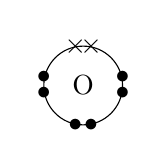
\begin{tikzpicture}
			\draw (0, 0) circle (0.5);
			\node at (0, 0) {O};
			\node at (0.5, -0.1) {$\bullet$};
			\node at (0.5, 0.1) {$\bullet$};
			\node at (-0.5, 0.1) {$\bullet$};
			\node at (-0.5, -0.1) {$\bullet$};
			\node at (0.1, -0.5) {$\bullet$};
			\node at (-0.1, -0.5) {$\bullet$};
			\node at (0.1, 0.5) {$\times$};
			\node at (-0.1, 0.5) {$\times$};
		\end{tikzpicture}
}}\right]^{2-}
$$

$$
\left[
	\vcenter{
		\hbox{
			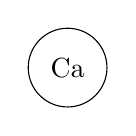
\begin{tikzpicture}
				\draw (0, 0) circle (0.5);
				\node at (0, 0) {Ca};
			\end{tikzpicture}
	}}
\right]^{2+}
\left[
\vcenter{
	\hbox{
		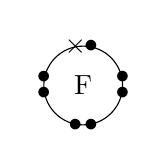
\begin{tikzpicture}
			\draw (0, 0) circle (0.5);
			\node at (0, 0) {F};
			\node at (0.5, -0.1) {$\bullet$};
			\node at (0.5, 0.1) {$\bullet$};
			\node at (-0.5, 0.1) {$\bullet$};
			\node at (-0.5, -0.1) {$\bullet$};
			\node at (0.1, -0.5) {$\bullet$};
			\node at (-0.1, -0.5) {$\bullet$};
			\node at (0.1, 0.5) {$\bullet$};
			\node at (-0.1, 0.5) {$\times$};
		\end{tikzpicture}
}}\right]^{-}
\left[
\vcenter{
	\hbox{
		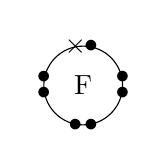
\begin{tikzpicture}
			\draw (0, 0) circle (0.5);
			\node at (0, 0) {F};
			\node at (0.5, -0.1) {$\bullet$};
			\node at (0.5, 0.1) {$\bullet$};
			\node at (-0.5, 0.1) {$\bullet$};
			\node at (-0.5, -0.1) {$\bullet$};
			\node at (0.1, -0.5) {$\bullet$};
			\node at (-0.1, -0.5) {$\bullet$};
			\node at (0.1, 0.5) {$\bullet$};
			\node at (-0.1, 0.5) {$\times$};
		\end{tikzpicture}
}}\right]^{-}
$$

\subsection{Metallic bonding}
\begin{point}
Define metallic bonding as the electrostatic attraction between postiive metal
ions and delocalised electrons
\end{point}
Self explanatory.

\subsection{Covalent bonding and coordinate (dative covalent) bonding}
\begin{point}
	Define covalent bonding as electrostatic attraction between the nuclei of two 
	atoms and a shared pair of electrons
	\begin{enumerate}[label=(\alph*)]
		\item Describe covalent bonding in molecules including:
			\begin{itemize}
				\item hydrogen, \ce{H2}
				\item oxygen, \ce{O2}
				\item nitrogen, \ce{N2}
				\item chlorine, \ce{Cl2}
				\item hydrogen chloride, \ce{HCl}
				\item carbon dioxide, \ce{CO2}
				\item ammonia, \ce{NH3}
				\item methane, \ce{CH4}
				\item ethane, \ce{C2H6}
				\item ethene, \ce{C2H4}
			\end{itemize}
		\item Understand that elements in period 3 can expand their octet including in the compounds
			sulfur dioxide, \ce{SO2}, phosphorus pentachloride, \ce{PCl5} , and sulfur hexafluoride, \ce{SF6}
		\item Describe coordinate (dative covalent) bonding, including in the reaction between ammonia and
			hydrogen chloride gases to form the ammonium ion, \ce{NH4+}, and in the \ce{Al2Cl6} molecule
	\end{enumerate}
\end{point}
